

\tikzset{every picture/.style={line width=0.75pt}} %set default line width to 0.75pt        

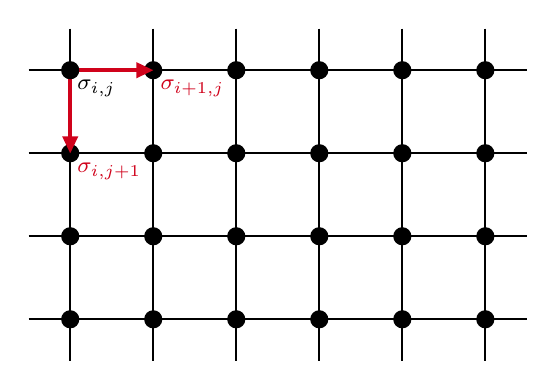
\begin{tikzpicture}[x=0.75pt,y=0.75pt,yscale=-1,xscale=1]
%uncomment if require: \path (0,300); %set diagram left start at 0, and has height of 300

%Shape: Grid [id:dp7936034410428405] 
\draw  [draw opacity=0][line width=0.75]  (50,40) -- (290,40) -- (290,200) -- (50,200) -- cycle ; \draw  [line width=0.75]  (70,40) -- (70,200)(110,40) -- (110,200)(150,40) -- (150,200)(190,40) -- (190,200)(230,40) -- (230,200)(270,40) -- (270,200) ; \draw  [line width=0.75]  (50,60) -- (290,60)(50,100) -- (290,100)(50,140) -- (290,140)(50,180) -- (290,180) ; \draw  [line width=0.75]   ;
%Shape: Circle [id:dp21137844160324193] 
\draw  [fill={rgb, 255:red, 0; green, 0; blue, 0 }  ,fill opacity=1 ] (106.13,60) .. controls (106.13,57.86) and (107.86,56.13) .. (110,56.13) .. controls (112.14,56.13) and (113.87,57.86) .. (113.87,60) .. controls (113.87,62.14) and (112.14,63.87) .. (110,63.87) .. controls (107.86,63.87) and (106.13,62.14) .. (106.13,60) -- cycle ;
%Shape: Circle [id:dp5614913237958086] 
\draw  [fill={rgb, 255:red, 0; green, 0; blue, 0 }  ,fill opacity=1 ] (146.13,60) .. controls (146.13,57.86) and (147.86,56.13) .. (150,56.13) .. controls (152.14,56.13) and (153.87,57.86) .. (153.87,60) .. controls (153.87,62.14) and (152.14,63.87) .. (150,63.87) .. controls (147.86,63.87) and (146.13,62.14) .. (146.13,60) -- cycle ;
%Shape: Circle [id:dp13112173645899605] 
\draw  [fill={rgb, 255:red, 0; green, 0; blue, 0 }  ,fill opacity=1 ] (186.13,60) .. controls (186.13,57.86) and (187.86,56.13) .. (190,56.13) .. controls (192.14,56.13) and (193.87,57.86) .. (193.87,60) .. controls (193.87,62.14) and (192.14,63.87) .. (190,63.87) .. controls (187.86,63.87) and (186.13,62.14) .. (186.13,60) -- cycle ;
%Shape: Circle [id:dp758519093575973] 
\draw  [fill={rgb, 255:red, 0; green, 0; blue, 0 }  ,fill opacity=1 ] (226.13,60) .. controls (226.13,57.86) and (227.86,56.13) .. (230,56.13) .. controls (232.14,56.13) and (233.87,57.86) .. (233.87,60) .. controls (233.87,62.14) and (232.14,63.87) .. (230,63.87) .. controls (227.86,63.87) and (226.13,62.14) .. (226.13,60) -- cycle ;
%Shape: Circle [id:dp9492458965331012] 
\draw  [fill={rgb, 255:red, 0; green, 0; blue, 0 }  ,fill opacity=1 ] (266.13,60) .. controls (266.13,57.86) and (267.86,56.13) .. (270,56.13) .. controls (272.14,56.13) and (273.87,57.86) .. (273.87,60) .. controls (273.87,62.14) and (272.14,63.87) .. (270,63.87) .. controls (267.86,63.87) and (266.13,62.14) .. (266.13,60) -- cycle ;
%Shape: Circle [id:dp41527636511725385] 
\draw  [fill={rgb, 255:red, 0; green, 0; blue, 0 }  ,fill opacity=1 ] (266.13,100) .. controls (266.13,97.86) and (267.86,96.13) .. (270,96.13) .. controls (272.14,96.13) and (273.87,97.86) .. (273.87,100) .. controls (273.87,102.14) and (272.14,103.87) .. (270,103.87) .. controls (267.86,103.87) and (266.13,102.14) .. (266.13,100) -- cycle ;
%Shape: Circle [id:dp7035046228897482] 
\draw  [fill={rgb, 255:red, 0; green, 0; blue, 0 }  ,fill opacity=1 ] (66.13,100) .. controls (66.13,97.86) and (67.86,96.13) .. (70,96.13) .. controls (72.14,96.13) and (73.87,97.86) .. (73.87,100) .. controls (73.87,102.14) and (72.14,103.87) .. (70,103.87) .. controls (67.86,103.87) and (66.13,102.14) .. (66.13,100) -- cycle ;
%Shape: Circle [id:dp8908755631753259] 
\draw  [fill={rgb, 255:red, 0; green, 0; blue, 0 }  ,fill opacity=1 ] (106.13,100) .. controls (106.13,97.86) and (107.86,96.13) .. (110,96.13) .. controls (112.14,96.13) and (113.87,97.86) .. (113.87,100) .. controls (113.87,102.14) and (112.14,103.87) .. (110,103.87) .. controls (107.86,103.87) and (106.13,102.14) .. (106.13,100) -- cycle ;
%Shape: Circle [id:dp6712289564140095] 
\draw  [fill={rgb, 255:red, 0; green, 0; blue, 0 }  ,fill opacity=1 ] (146.13,100) .. controls (146.13,97.86) and (147.86,96.13) .. (150,96.13) .. controls (152.14,96.13) and (153.87,97.86) .. (153.87,100) .. controls (153.87,102.14) and (152.14,103.87) .. (150,103.87) .. controls (147.86,103.87) and (146.13,102.14) .. (146.13,100) -- cycle ;
%Shape: Circle [id:dp913957826655591] 
\draw  [fill={rgb, 255:red, 0; green, 0; blue, 0 }  ,fill opacity=1 ] (186.13,100) .. controls (186.13,97.86) and (187.86,96.13) .. (190,96.13) .. controls (192.14,96.13) and (193.87,97.86) .. (193.87,100) .. controls (193.87,102.14) and (192.14,103.87) .. (190,103.87) .. controls (187.86,103.87) and (186.13,102.14) .. (186.13,100) -- cycle ;
%Shape: Circle [id:dp580135342118122] 
\draw  [fill={rgb, 255:red, 0; green, 0; blue, 0 }  ,fill opacity=1 ] (226.13,100) .. controls (226.13,97.86) and (227.86,96.13) .. (230,96.13) .. controls (232.14,96.13) and (233.87,97.86) .. (233.87,100) .. controls (233.87,102.14) and (232.14,103.87) .. (230,103.87) .. controls (227.86,103.87) and (226.13,102.14) .. (226.13,100) -- cycle ;
%Shape: Circle [id:dp06843162051040319] 
\draw  [fill={rgb, 255:red, 0; green, 0; blue, 0 }  ,fill opacity=1 ] (66.13,140) .. controls (66.13,137.86) and (67.86,136.13) .. (70,136.13) .. controls (72.14,136.13) and (73.87,137.86) .. (73.87,140) .. controls (73.87,142.14) and (72.14,143.87) .. (70,143.87) .. controls (67.86,143.87) and (66.13,142.14) .. (66.13,140) -- cycle ;
%Shape: Circle [id:dp03818342408502351] 
\draw  [fill={rgb, 255:red, 0; green, 0; blue, 0 }  ,fill opacity=1 ] (106.13,140) .. controls (106.13,137.86) and (107.86,136.13) .. (110,136.13) .. controls (112.14,136.13) and (113.87,137.86) .. (113.87,140) .. controls (113.87,142.14) and (112.14,143.87) .. (110,143.87) .. controls (107.86,143.87) and (106.13,142.14) .. (106.13,140) -- cycle ;
%Shape: Circle [id:dp057567593025961816] 
\draw  [fill={rgb, 255:red, 0; green, 0; blue, 0 }  ,fill opacity=1 ] (146.13,140) .. controls (146.13,137.86) and (147.86,136.13) .. (150,136.13) .. controls (152.14,136.13) and (153.87,137.86) .. (153.87,140) .. controls (153.87,142.14) and (152.14,143.87) .. (150,143.87) .. controls (147.86,143.87) and (146.13,142.14) .. (146.13,140) -- cycle ;
%Shape: Circle [id:dp3547020763113766] 
\draw  [fill={rgb, 255:red, 0; green, 0; blue, 0 }  ,fill opacity=1 ] (186.13,140) .. controls (186.13,137.86) and (187.86,136.13) .. (190,136.13) .. controls (192.14,136.13) and (193.87,137.86) .. (193.87,140) .. controls (193.87,142.14) and (192.14,143.87) .. (190,143.87) .. controls (187.86,143.87) and (186.13,142.14) .. (186.13,140) -- cycle ;
%Shape: Circle [id:dp27735818122011624] 
\draw  [fill={rgb, 255:red, 0; green, 0; blue, 0 }  ,fill opacity=1 ] (226.13,140) .. controls (226.13,137.86) and (227.86,136.13) .. (230,136.13) .. controls (232.14,136.13) and (233.87,137.86) .. (233.87,140) .. controls (233.87,142.14) and (232.14,143.87) .. (230,143.87) .. controls (227.86,143.87) and (226.13,142.14) .. (226.13,140) -- cycle ;
%Shape: Circle [id:dp7327768001985178] 
\draw  [fill={rgb, 255:red, 0; green, 0; blue, 0 }  ,fill opacity=1 ] (266.13,140) .. controls (266.13,137.86) and (267.86,136.13) .. (270,136.13) .. controls (272.14,136.13) and (273.87,137.86) .. (273.87,140) .. controls (273.87,142.14) and (272.14,143.87) .. (270,143.87) .. controls (267.86,143.87) and (266.13,142.14) .. (266.13,140) -- cycle ;
%Shape: Circle [id:dp8732521224319985] 
\draw  [fill={rgb, 255:red, 0; green, 0; blue, 0 }  ,fill opacity=1 ] (66.13,180) .. controls (66.13,177.86) and (67.86,176.13) .. (70,176.13) .. controls (72.14,176.13) and (73.87,177.86) .. (73.87,180) .. controls (73.87,182.14) and (72.14,183.87) .. (70,183.87) .. controls (67.86,183.87) and (66.13,182.14) .. (66.13,180) -- cycle ;
%Shape: Circle [id:dp18708605081031293] 
\draw  [fill={rgb, 255:red, 0; green, 0; blue, 0 }  ,fill opacity=1 ] (106.13,180) .. controls (106.13,177.86) and (107.86,176.13) .. (110,176.13) .. controls (112.14,176.13) and (113.87,177.86) .. (113.87,180) .. controls (113.87,182.14) and (112.14,183.87) .. (110,183.87) .. controls (107.86,183.87) and (106.13,182.14) .. (106.13,180) -- cycle ;
%Shape: Circle [id:dp07061774773338303] 
\draw  [fill={rgb, 255:red, 0; green, 0; blue, 0 }  ,fill opacity=1 ] (146.13,180) .. controls (146.13,177.86) and (147.86,176.13) .. (150,176.13) .. controls (152.14,176.13) and (153.87,177.86) .. (153.87,180) .. controls (153.87,182.14) and (152.14,183.87) .. (150,183.87) .. controls (147.86,183.87) and (146.13,182.14) .. (146.13,180) -- cycle ;
%Shape: Circle [id:dp9207789260011581] 
\draw  [fill={rgb, 255:red, 0; green, 0; blue, 0 }  ,fill opacity=1 ] (186.13,180) .. controls (186.13,177.86) and (187.86,176.13) .. (190,176.13) .. controls (192.14,176.13) and (193.87,177.86) .. (193.87,180) .. controls (193.87,182.14) and (192.14,183.87) .. (190,183.87) .. controls (187.86,183.87) and (186.13,182.14) .. (186.13,180) -- cycle ;
%Shape: Circle [id:dp2505566533900382] 
\draw  [fill={rgb, 255:red, 0; green, 0; blue, 0 }  ,fill opacity=1 ] (226.13,180) .. controls (226.13,177.86) and (227.86,176.13) .. (230,176.13) .. controls (232.14,176.13) and (233.87,177.86) .. (233.87,180) .. controls (233.87,182.14) and (232.14,183.87) .. (230,183.87) .. controls (227.86,183.87) and (226.13,182.14) .. (226.13,180) -- cycle ;
%Shape: Circle [id:dp8687644835716081] 
\draw  [fill={rgb, 255:red, 0; green, 0; blue, 0 }  ,fill opacity=1 ] (266.13,180) .. controls (266.13,177.86) and (267.86,176.13) .. (270,176.13) .. controls (272.14,176.13) and (273.87,177.86) .. (273.87,180) .. controls (273.87,182.14) and (272.14,183.87) .. (270,183.87) .. controls (267.86,183.87) and (266.13,182.14) .. (266.13,180) -- cycle ;
%Straight Lines [id:da1479615822199637] 
\draw [color={rgb, 255:red, 208; green, 2; blue, 27 }  ,draw opacity=1 ][line width=1.5]    (70,60) -- (106,60) ;
\draw [shift={(110,60)}, rotate = 180] [fill={rgb, 255:red, 208; green, 2; blue, 27 }  ,fill opacity=1 ][line width=0.08]  [draw opacity=0] (8.13,-3.9) -- (0,0) -- (8.13,3.9) -- cycle    ;
%Straight Lines [id:da4838541935499793] 
\draw [color={rgb, 255:red, 208; green, 2; blue, 27 }  ,draw opacity=1 ][line width=1.5]    (70,60) -- (70,96) ;
\draw [shift={(70,100)}, rotate = 270] [fill={rgb, 255:red, 208; green, 2; blue, 27 }  ,fill opacity=1 ][line width=0.08]  [draw opacity=0] (8.13,-3.9) -- (0,0) -- (8.13,3.9) -- cycle    ;
%Shape: Circle [id:dp012956131714181307] 
\draw  [fill={rgb, 255:red, 0; green, 0; blue, 0 }  ,fill opacity=1 ] (66.13,60) .. controls (66.13,57.86) and (67.86,56.13) .. (70,56.13) .. controls (72.14,56.13) and (73.87,57.86) .. (73.87,60) .. controls (73.87,62.14) and (72.14,63.87) .. (70,63.87) .. controls (67.86,63.87) and (66.13,62.14) .. (66.13,60) -- cycle ;

% Text Node
\draw (72,63.4) node [anchor=north west][inner sep=0.75pt]  [font=\footnotesize,color={rgb, 255:red, 0; green, 0; blue, 0 }  ,opacity=1 ]  {$\sigma_{i,j}$};
% Text Node
\draw (72,103.4) node [anchor=north west][inner sep=0.75pt]  [font=\footnotesize,color={rgb, 255:red, 208; green, 2; blue, 27 }  ,opacity=1 ]  {$\sigma_{i,j+1}$};
% Text Node
\draw (112,63.4) node [anchor=north west][inner sep=0.75pt]  [font=\footnotesize,color={rgb, 255:red, 208; green, 2; blue, 27 }  ,opacity=1 ]  {$\sigma_{i+1,j}$};


\end{tikzpicture}
